% Euclidean Handout Number Two Fall 2013
\documentclass{tufte-handout}

%\geometry{showframe}% for debugging purposes -- displays the margins

%%%% Packages to make things pretty
\usepackage{amsmath,amsthm}
\usepackage{booktabs}
\usepackage{graphicx}
\setkeys{Gin}{width=\linewidth,totalheight=\textheight,keepaspectratio}
\graphicspath{{graphics/}}
\usepackage{units}
\usepackage{fancyvrb}
\fvset{fontsize=\normalsize}
\usepackage{multicol}
\usepackage{pdfpages}

%%%% Theorem Evironments
\theoremstyle{definition}
\swapnumbers
\newtheorem{problem}{Problem}[section]
\newtheorem{conjecture}[problem]{Conjecture}
\newtheorem*{definition}{Definition}
\newtheorem*{theorem}{Theorem}
\newtheorem{question}[problem]{Question}
\newtheorem{challenge}[problem]{Challenge}
\newtheorem*{postulate}{Postulate}

%%%%%

\title{Euclidean Geometry:\\An Introduction to Mathematical Work}
\author[]{Math 3600, Fall 2013}
\date{7 September}

\begin{document}

\maketitle

\begin{marginfigure}
    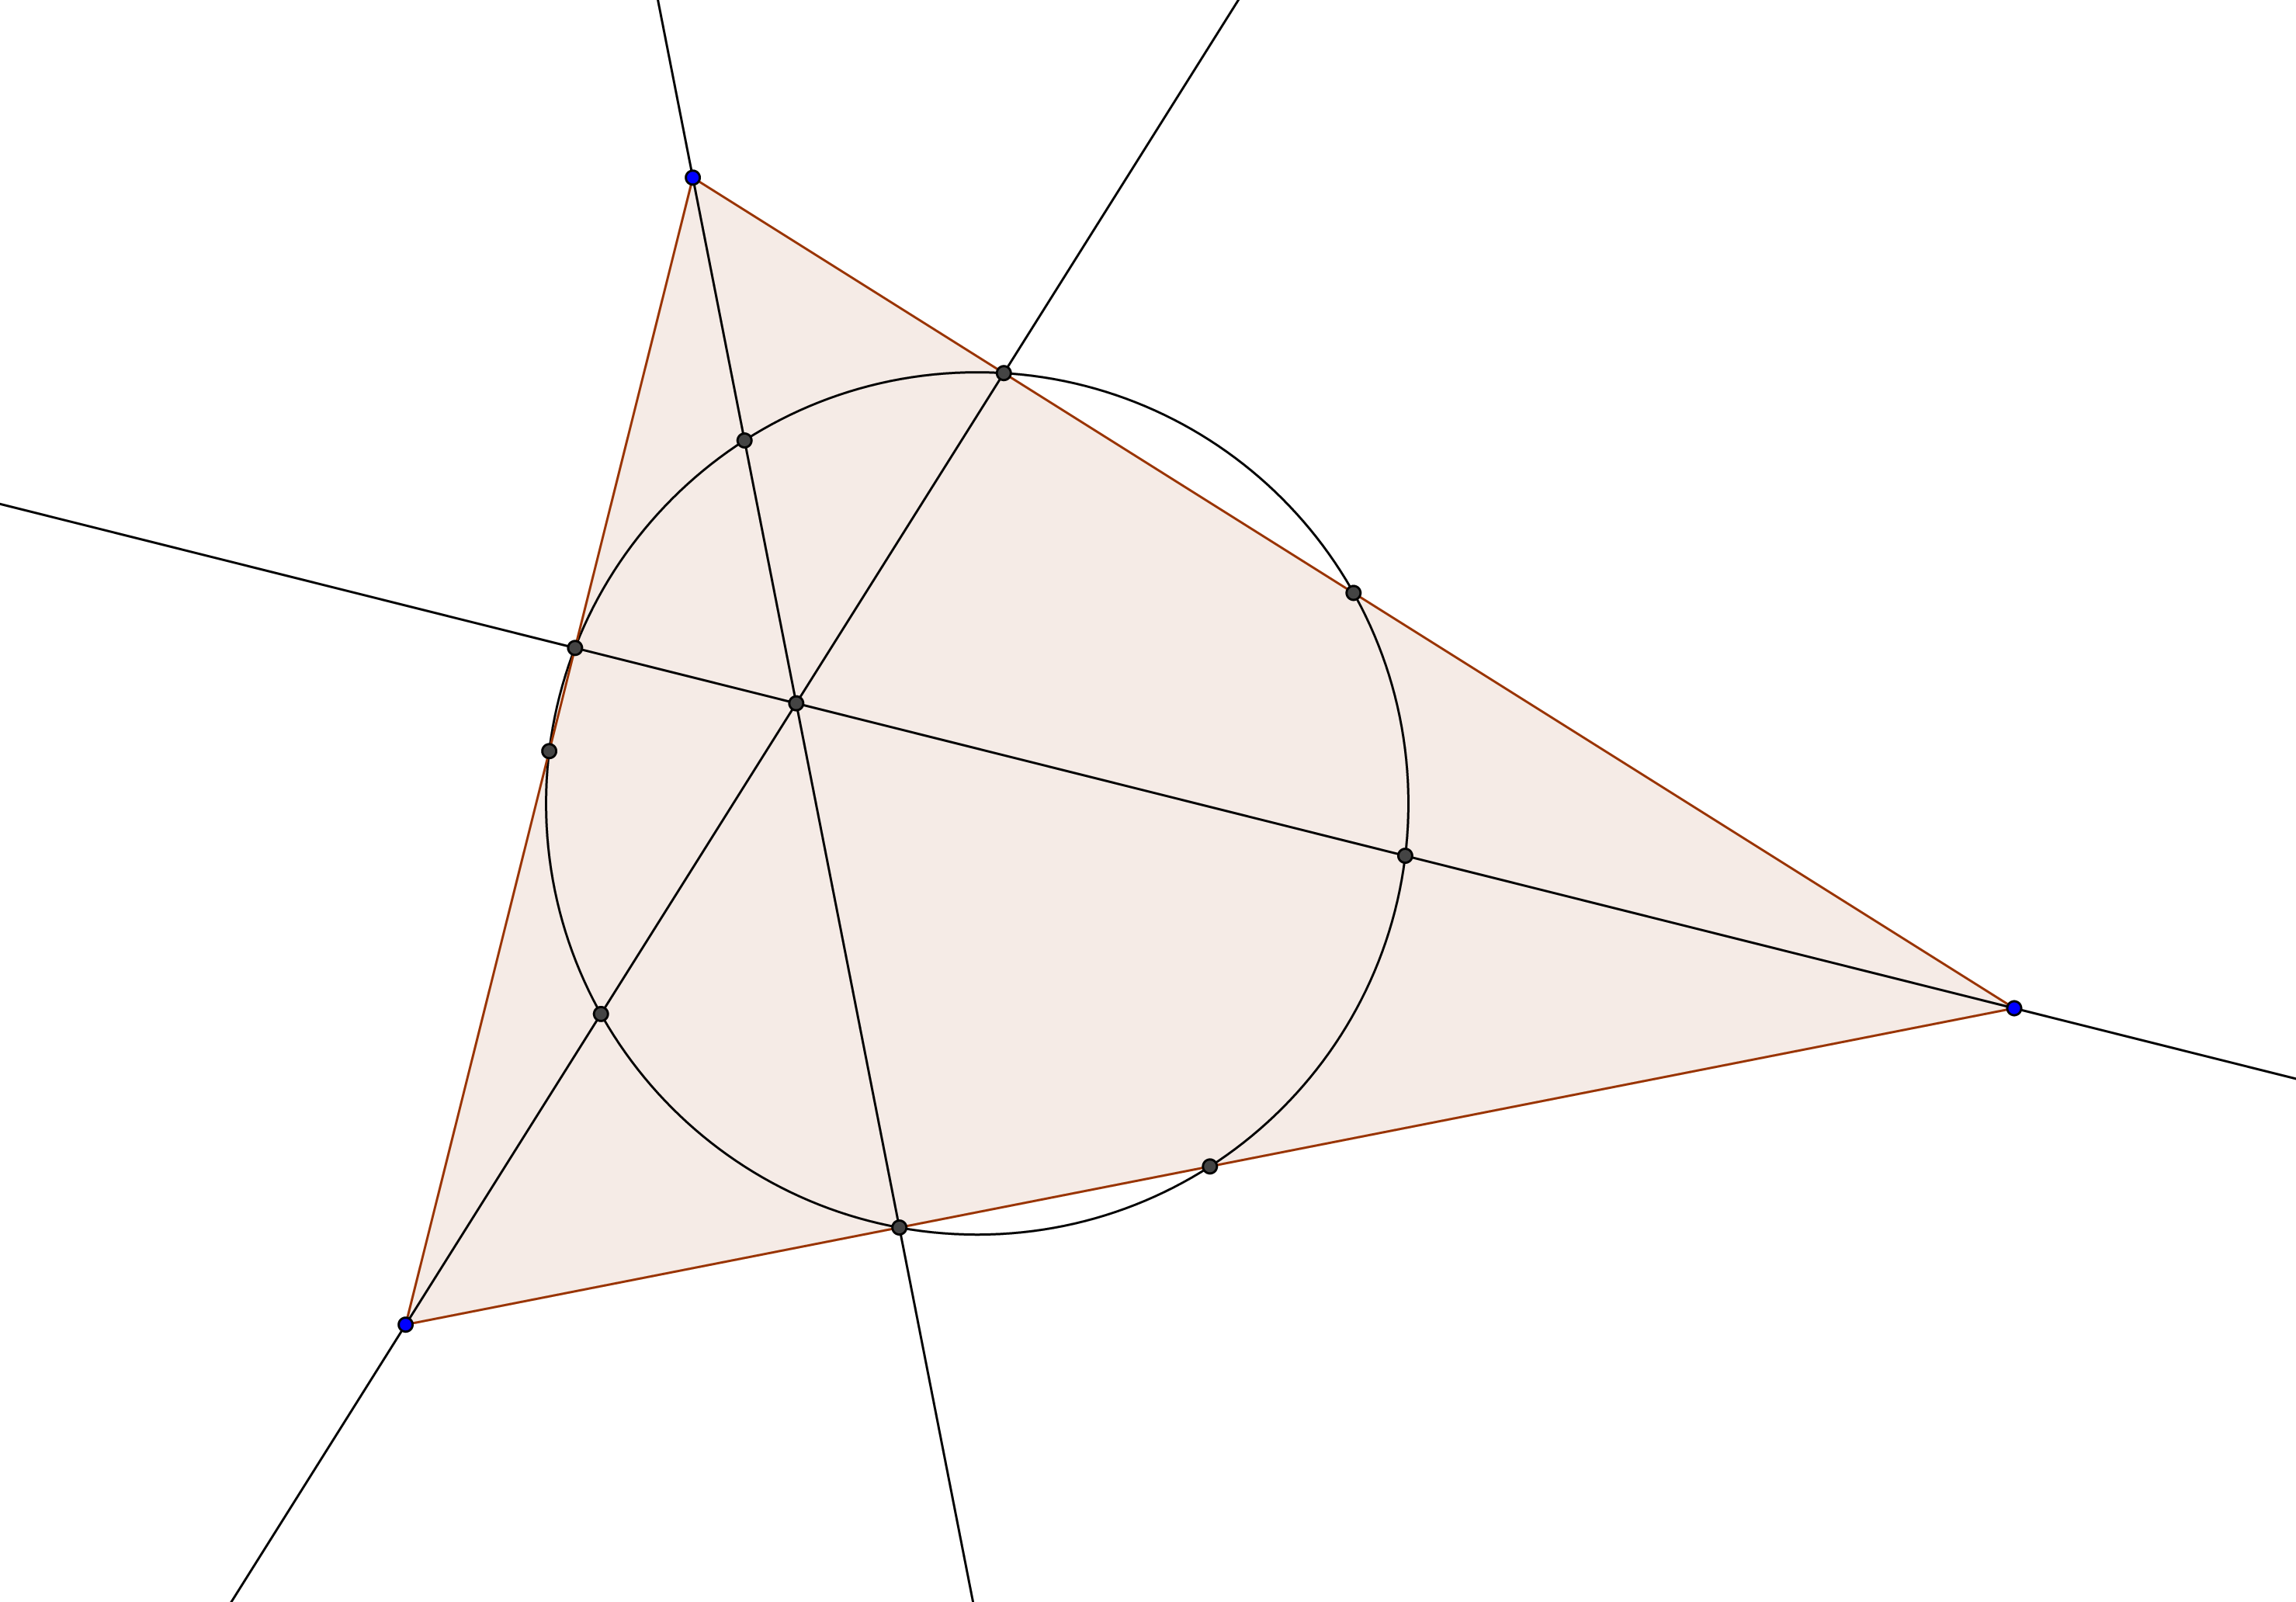
\includegraphics{NPC}
\end{marginfigure}

\setcounter{section}{2}
\section{The Geometry of Kites}

Now we turn our attention to a different special class of quadrilaterals: \emph{kites}. 

\begin{definition}\label{defn:quad-sides-type}
Two sides of a quadrilateral are called \emph{adjacent} when they share a vertex and \emph{opposite} if they do not.
\end{definition}

\marginnote[-10pt]{Again, here are some new definitions. To make sense of them, try creating some examples and some ``non-examples.''}

\begin{definition}\label{defn:kite}
A \emph{kite} is a quadrilateral with two pairs of adjacent and congruent sides.
\end{definition}

\newthought{Notice that} a rhombus is always a kite.
\marginnote{This is a theorem (and its proof). Can you write it out so it looks like a formal theorem statment?}
The reason is that if all four sides are mutually congruent, then we can pick any way we like to divide the sides into adjacent pairs (there are only two ways), and these pairs will consist of congruent sides.

Sometimes a proof has features that can be carried over to other situations. 
In this assignment, you should try to build on the ideas we have developed in studying rhombi in this new situation.
Each of the below is an adaptation of a statement we have for rhombi.

\begin{conjecture}\label{conj:kite-opp-angles} 
Pairs of opposite angles in a kite are congruent.
\end{conjecture}

\begin{conjecture}\label{conj:kite-diagonals-cross} 
The diagonals of a kite must cross.
\end{conjecture}

\begin{problem}\label{prob:construct-kites} 
Give a construction (with proof) of a kite. 
How general is your construction? 
\end{problem}

\begin{conjecture}\label{conj:kite-is-parallelogram} 
If $ABCD$ is a kite, then it is a parallelogram.
\end{conjecture}

\begin{conjecture}\label{conj:kite-diagonals-perpendicular} 
If the diagonals of a kite meet, then they meet at a right angle.
\end{conjecture}

\vfill
\end{document}
